\section{Evaluation}\label{sec:eval}

We evaluated our mpi, hybrid implementations of each algorithm (rs, block, fw) by doing strong scaling studies across a range of problem sizes. For rs and block we used a baseline of \rs{omp} and for fw we used a baseline of \fw{omp}. For rs and block we also did weak scaling studies for with a constant work of problem size $n=500$.

\subsection{RS}

\subsubsection{MPI}

\begin{figure}[ht]
\centering
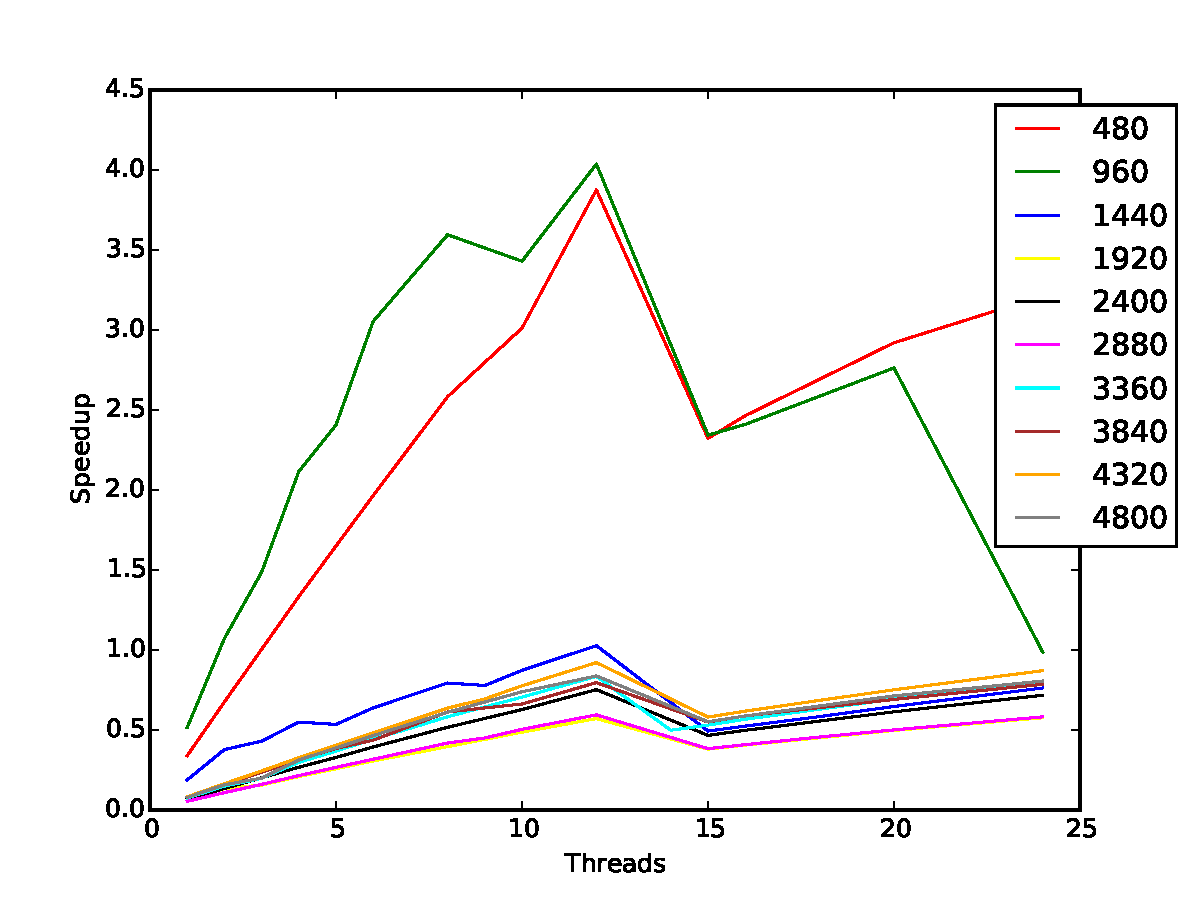
\includegraphics[width=0.5\textwidth]{plots/strong_rs-mpi_baseline-rs-omp--1.pdf}
\caption{Strong scaling for rs-mpi with a baseline of rs-omp}
\label{strong-rs-mpi}
\end{figure}

\begin{figure}[ht]
\centering
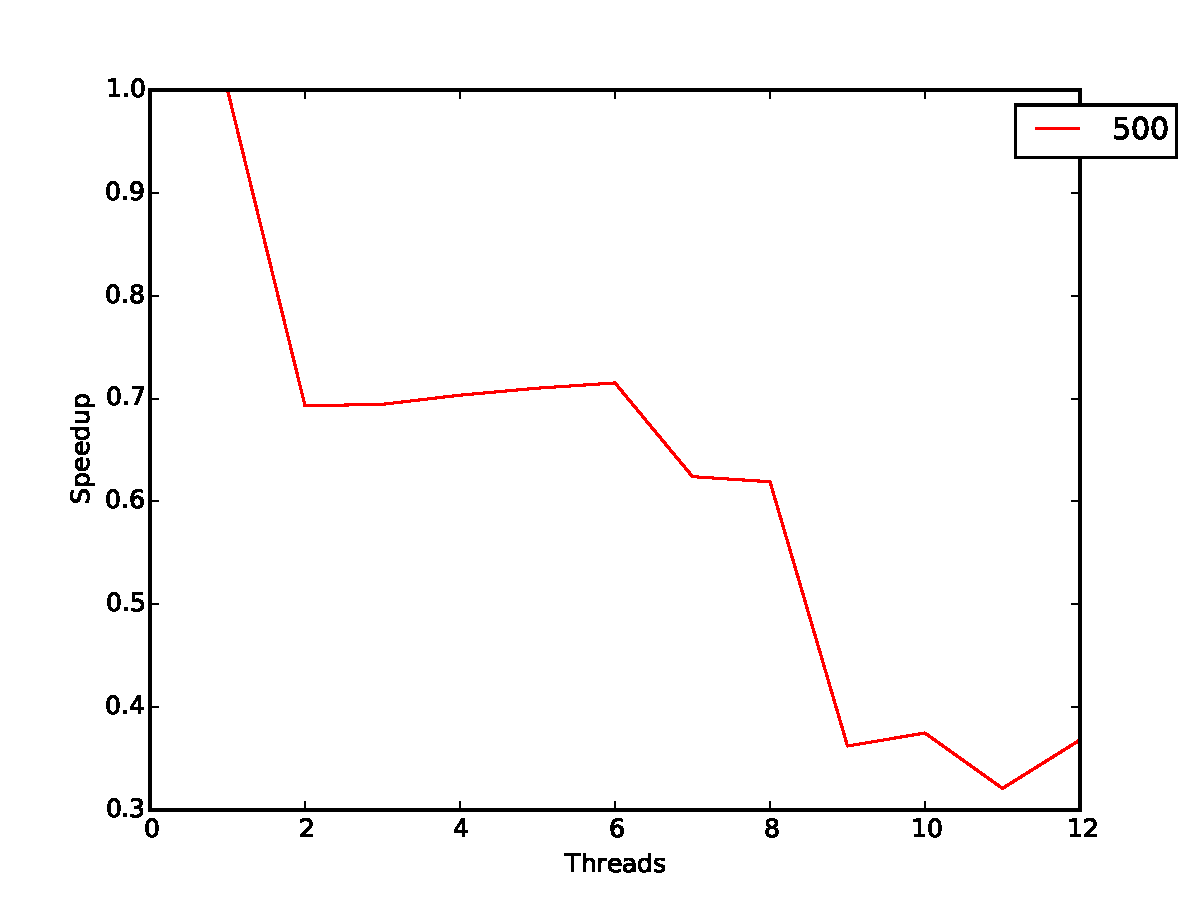
\includegraphics[width=0.5\textwidth]{plots/weak_rs-mpi.pdf}
\caption{Weak scaling for rs-mpi (baseline of itself).}
\label{weak-rs-mpi}
\end{figure}

\subsubsection{Hybrid}

\begin{figure}[ht]
\centering
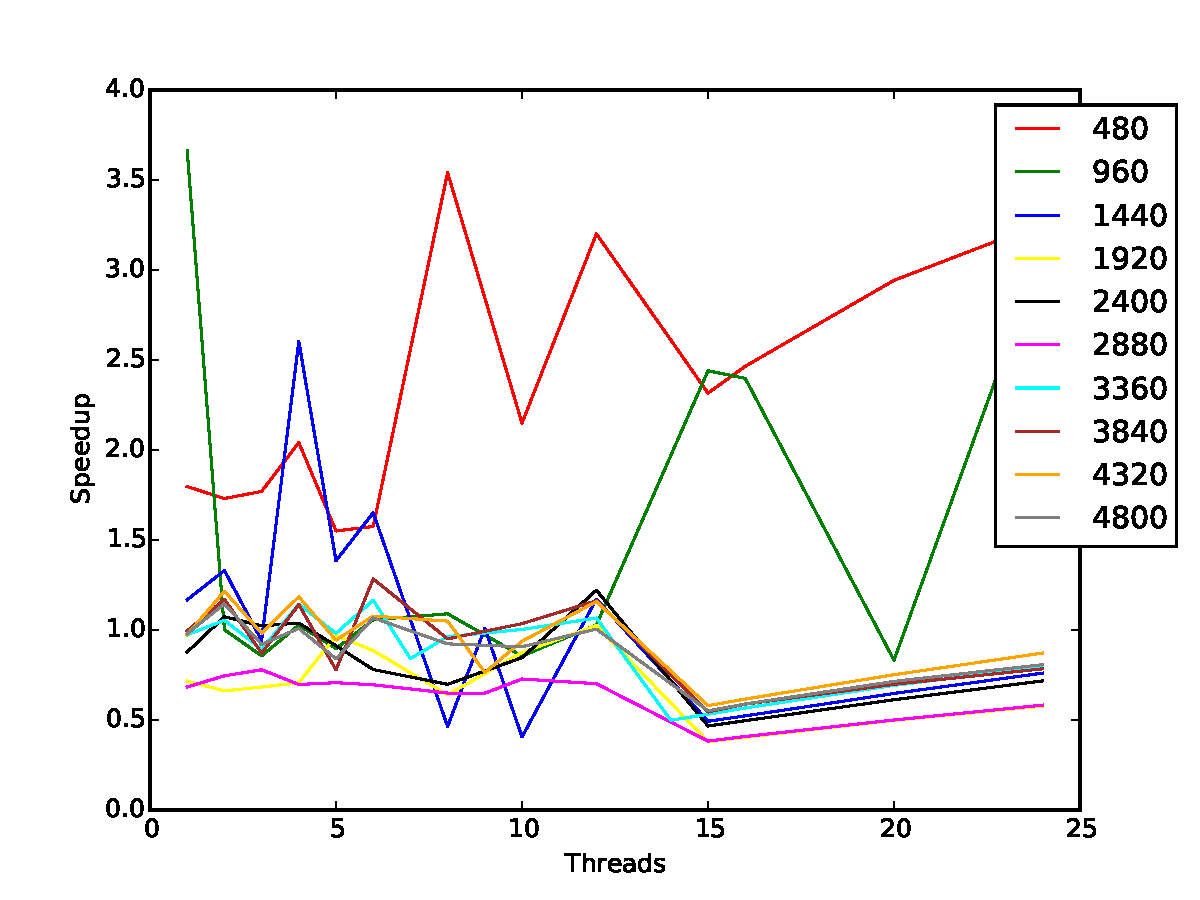
\includegraphics[width=0.5\textwidth]{plots/strong_rs-hybrid_baseline-rs-omp--1.pdf}
\caption{Strong scaling for rs-hybrid with a baseline of rs-omp}
\label{strong-rs-hybrid}
\end{figure}

\begin{figure}[ht]
\centering
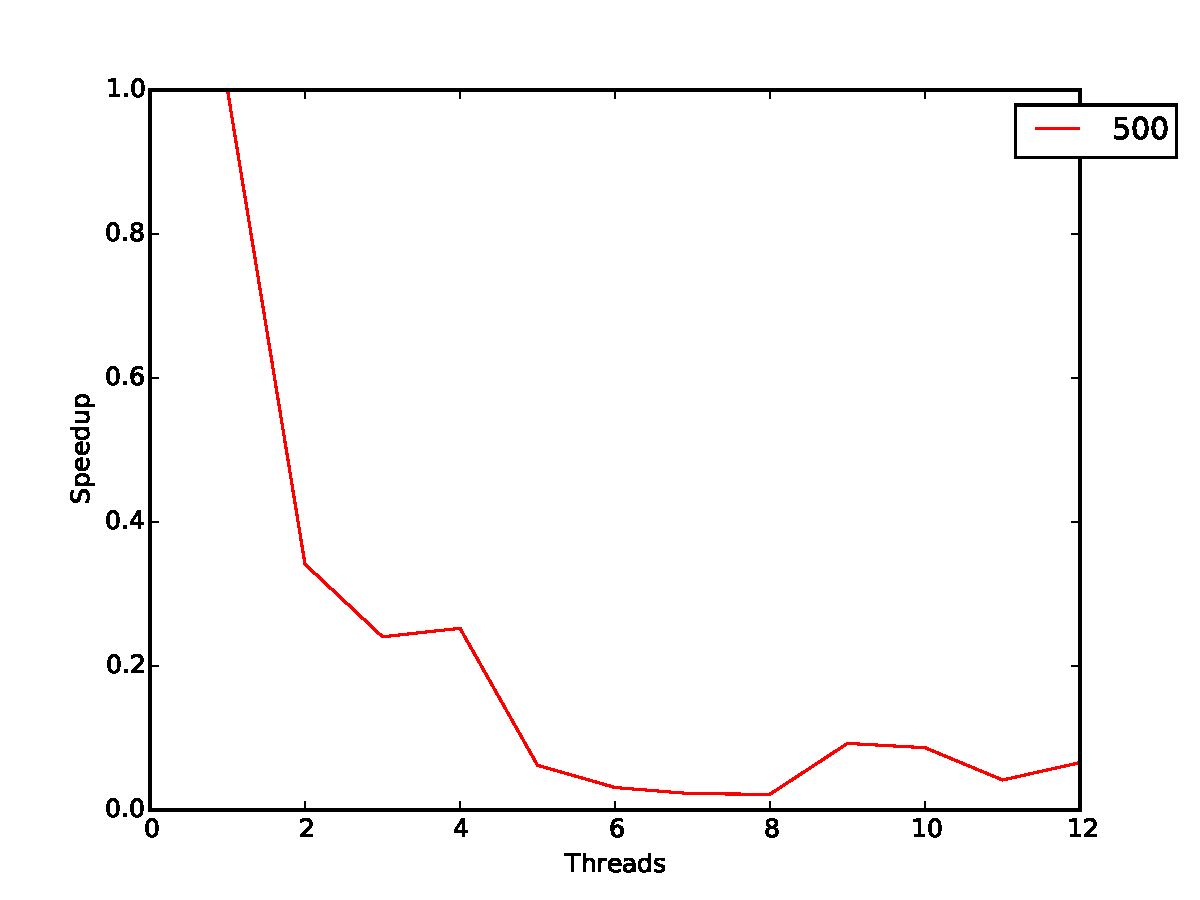
\includegraphics[width=0.5\textwidth]{plots/weak_rs-hybrid.pdf}
\caption{Weak scaling for rs-hybrid (baseline of itself).}
\label{weak-rs-hybrid}
\end{figure}


\subsection{Block}

\subsubsection{MPI}

\begin{figure}[ht]
\centering
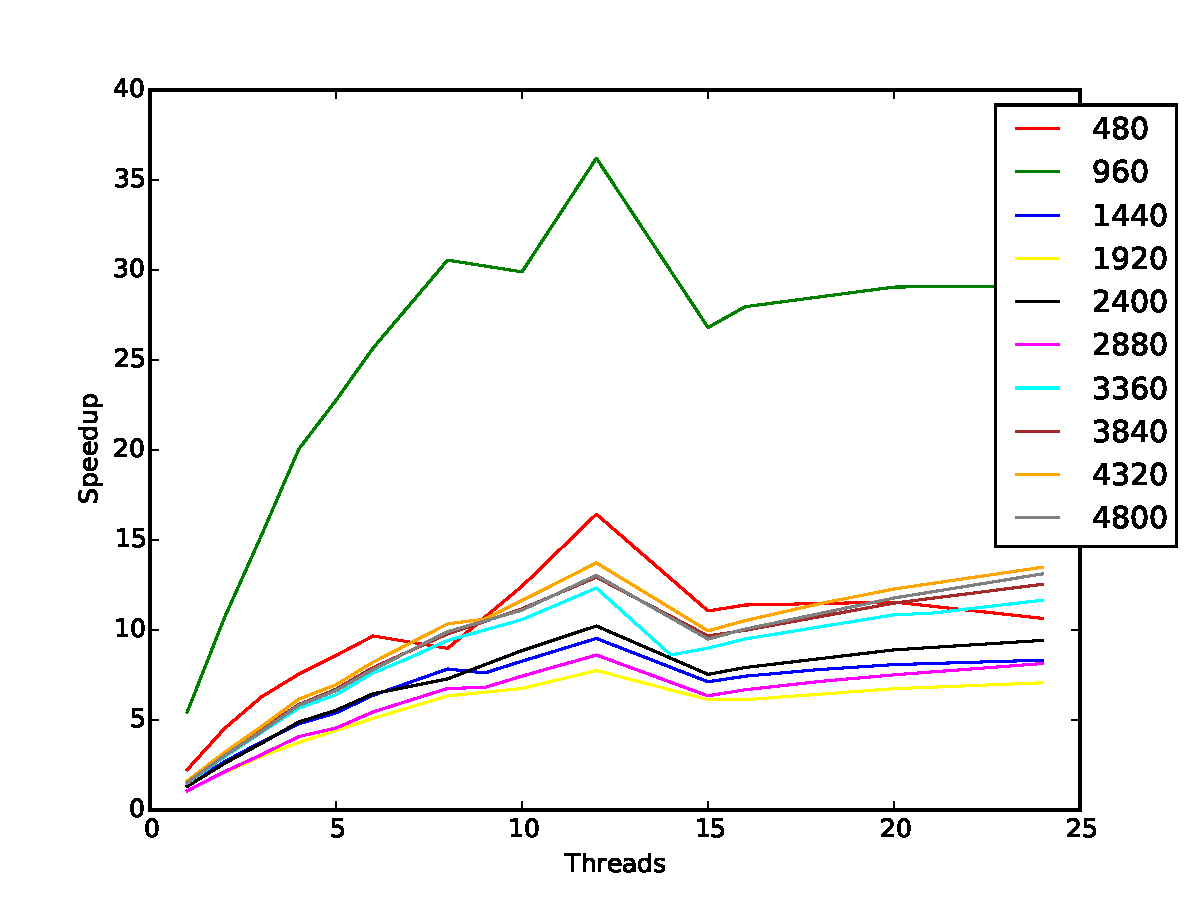
\includegraphics[width=0.5\textwidth]{plots/strong_block-mpi_baseline-rs-omp--1.pdf}
\caption{Strong scaling for block-mpi with a baseline of rs-omp}
\label{strong-block-mpi}
\end{figure}

\begin{figure}[ht]
\centering
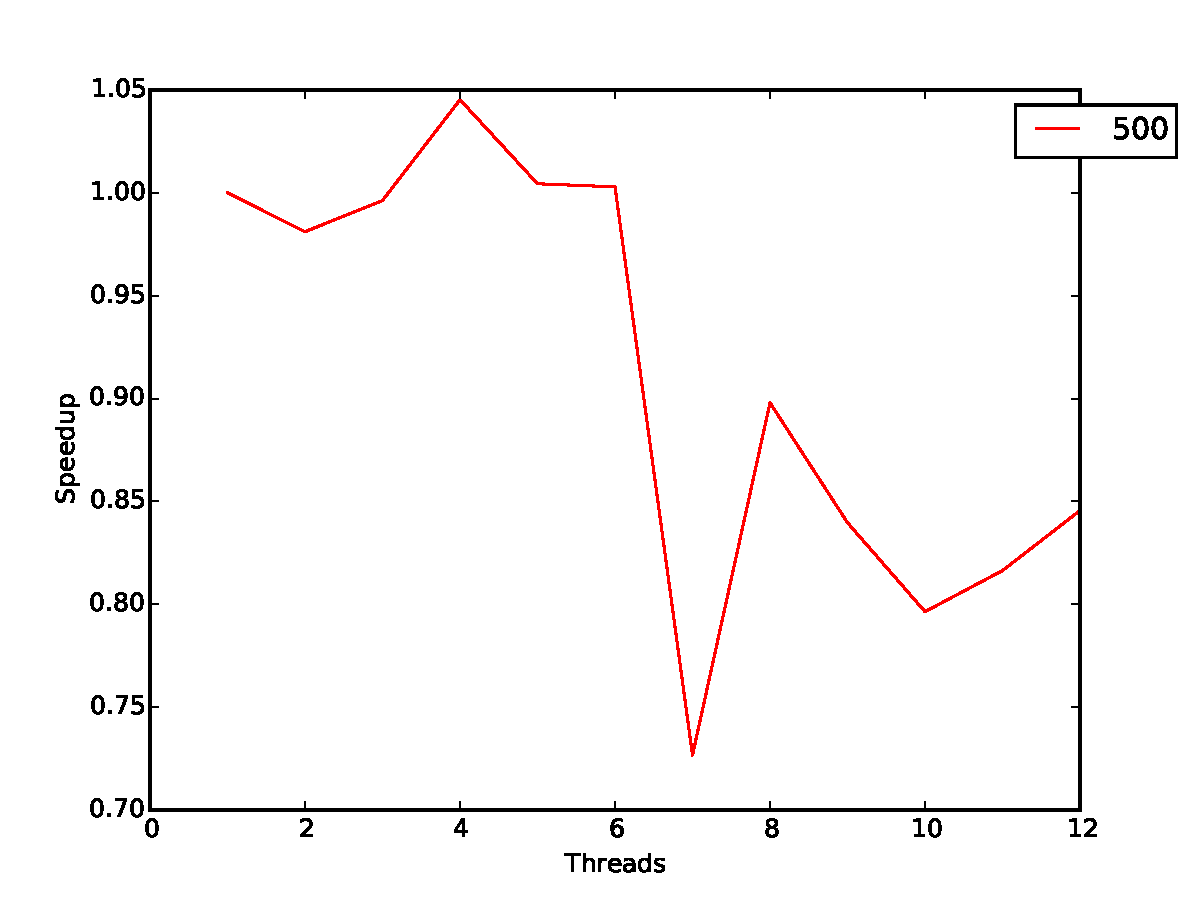
\includegraphics[width=0.5\textwidth]{plots/weak_block-mpi.pdf}
\caption{Weak scaling for block-mpi (baseline of itself).}
\label{weak-block-mpi}
\end{figure}

\subsubsection{Hybrid}

\begin{figure}[ht]
\centering
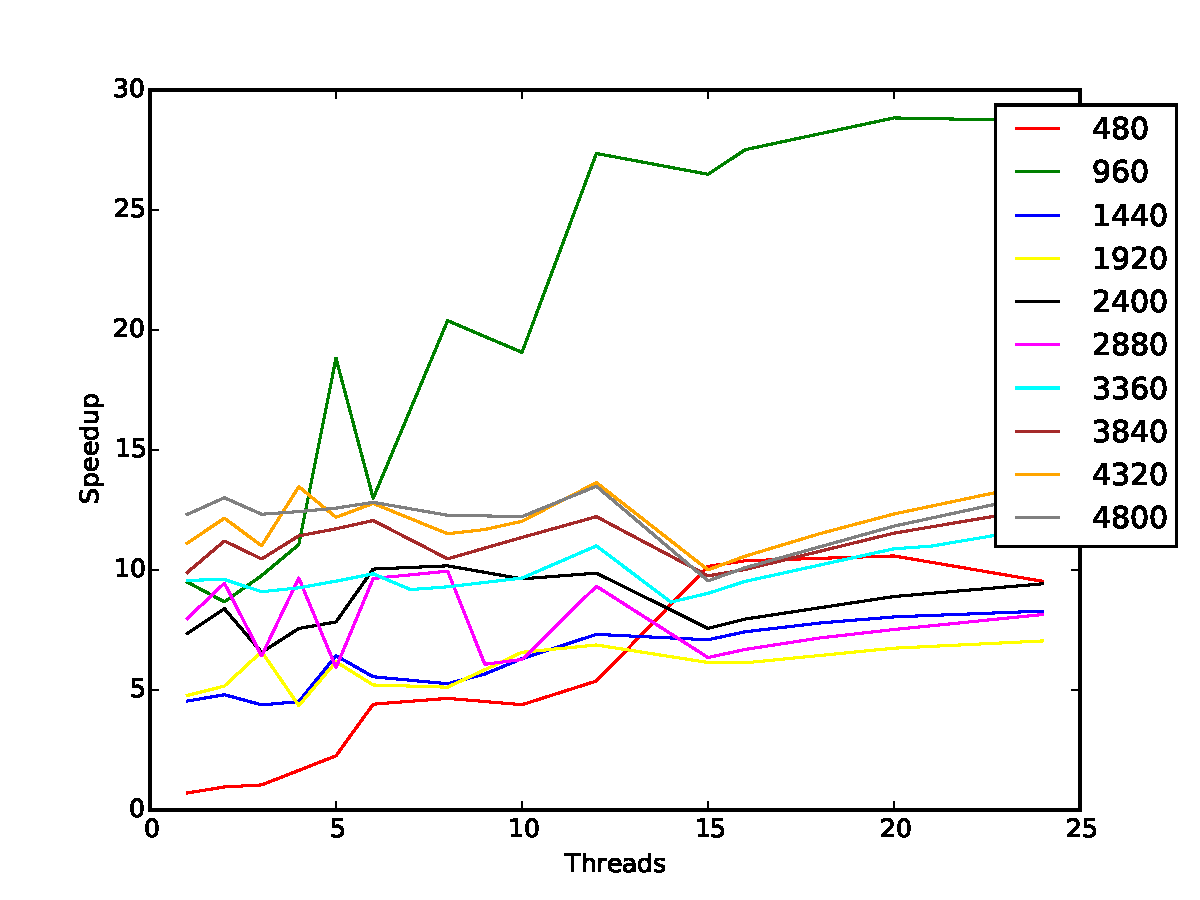
\includegraphics[width=0.5\textwidth]{plots/strong_block-hybrid_baseline-rs-omp--1.pdf}
\caption{Strong scaling for block-hybrid with a baseline of rs-omp}
\label{strong-block-hybrid}
\end{figure}

\begin{figure}[ht]
\centering
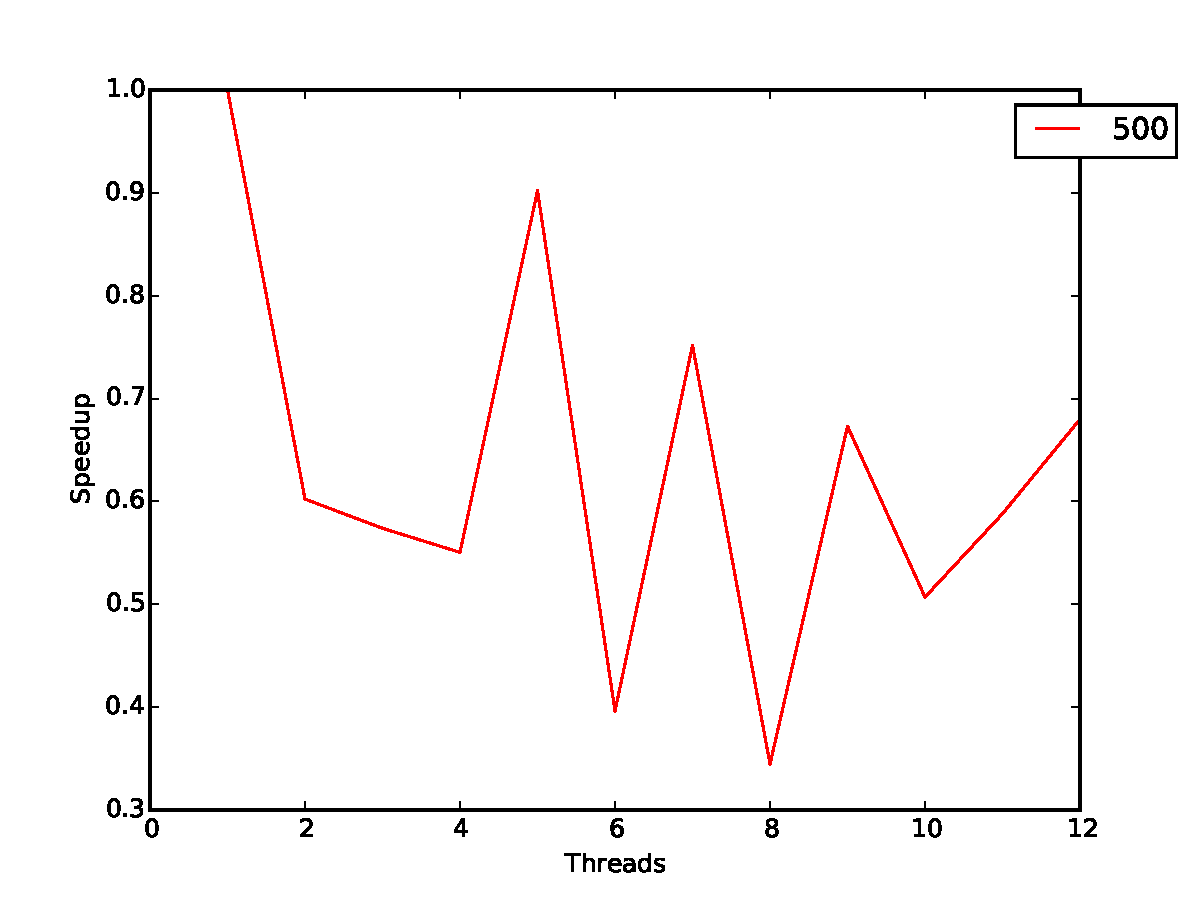
\includegraphics[width=0.5\textwidth]{plots/weak_block-hybrid.pdf}
\caption{Weak scaling for block-hybrid (baseline of itself).}
\label{weak-block-hybrid}
\end{figure}

\subsection{FW}

\subsubsection{MPI}

\begin{figure}[ht]
\centering
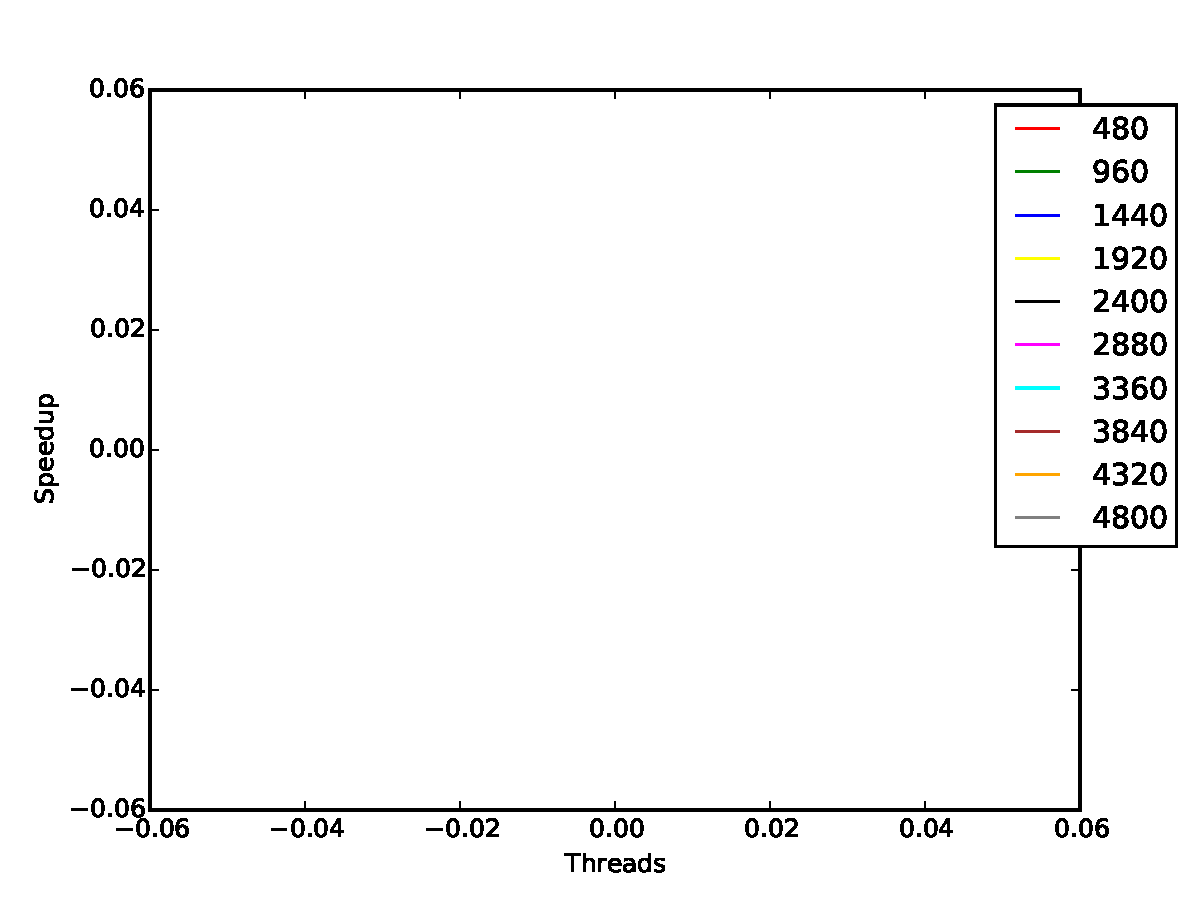
\includegraphics[width=0.5\textwidth]{plots/strong_fw-mpi_baseline-fw-omp--1.pdf}
\caption{Strong scaling for fw-mpi with a baseline of fw-omp}
\label{strong-fw-mpi}
\end{figure}

\subsubsection{Hybrid}

\begin{figure}[ht]
\centering
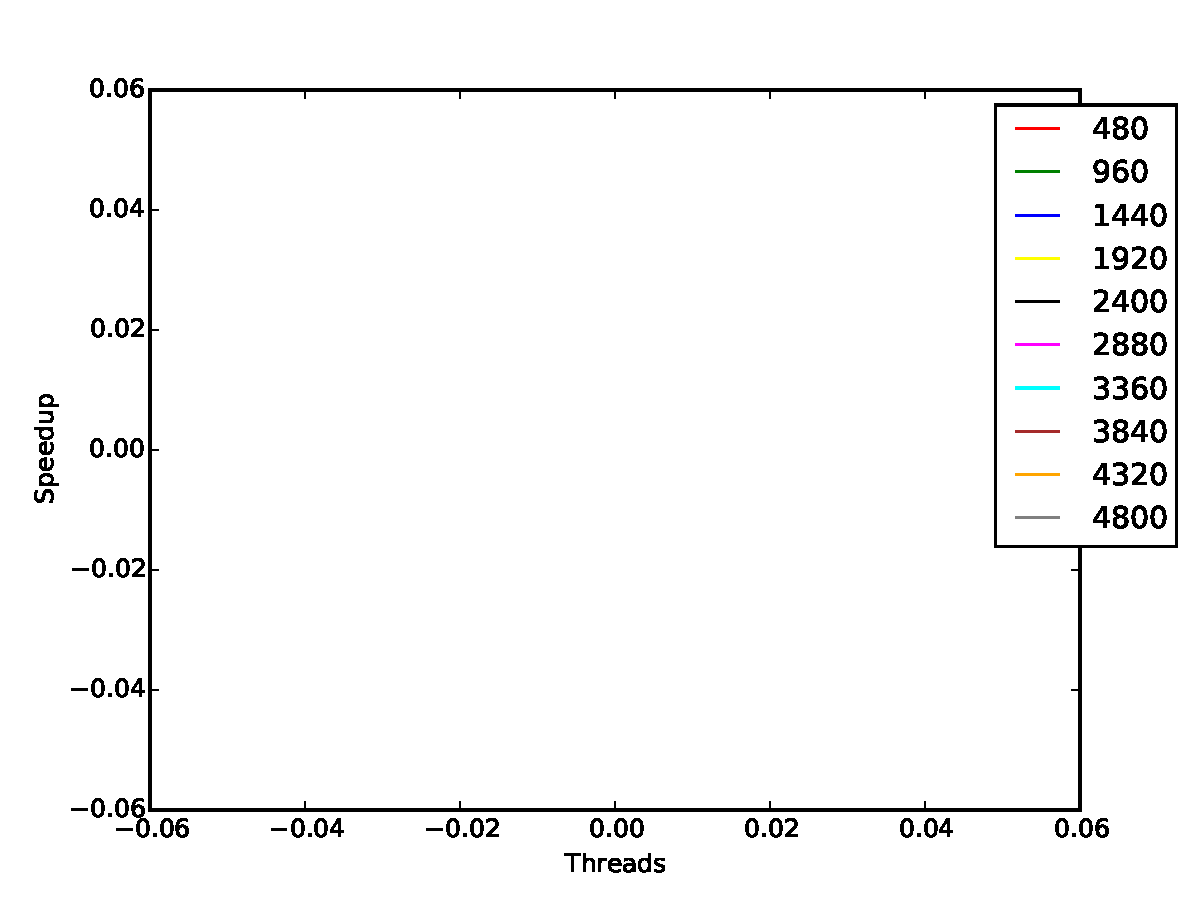
\includegraphics[width=0.5\textwidth]{plots/strong_fw-hybrid_baseline-fw-omp--1.pdf}
\caption{Strong scaling for fw-hybrid with a baseline of fw-omp}
\label{strong-fw-mpi}
\end{figure}
